\documentclass[a4paper,12pt,landscape]{article}
\usepackage{graphicx}
    \graphicspath{ {./Graphics/} }
\usepackage[top=1.5cm,bottom=1.5cm,left=1cm,right=1cm,marginparwidth=1cm]{geometry}
\usepackage{xcolor}
\usepackage{fancyhdr}
\usepackage{tikz}
    \usetikzlibrary{calc}
\usepackage{fontspec}
\usepackage{titlesec}
\setmainfont{WorkSans}[
    Path=./FontFiles/WorkSansFiles/,
    Extension = .ttf,
    UprightFont=*-Regular,
    BoldFont=*-Bold,
    ItalicFont=*-Italic,
    BoldItalicFont=*-BoldItalic,
    SlantedFont=*-ExtraBold
]
\definecolor{natblå}{HTML}{003255}
\definecolor{søblå}{HTML}{4678C8}
\definecolor{flammefarvet}{HTML}{FF733C}
\definecolor{syren}{HTML}{9182C8}
\definecolor{korngul}{HTML}{FFB91E}
\definecolor{efterårsrød}{HTML}{D22832}
\definecolor{græsgrøn}{HTML}{7DC855}
\definecolor{granit}{HTML}{7D878C}
\definecolor{skumringsblå}{HTML}{5F8CB4}
% SINCE ORIGINAL TEMPLATE USES TWO BOLD THICKNESSES WE HIJACK THE SLANTED FONT FAMILY TO REUSE AS EXTRABOLD INSTEAD

\renewcommand{\title}[1]{\noindent{\color{natblå}\normalfont\huge\slshape{#1}}}

\titleformat{\section}
{\color{natblå}\normalfont\LARGE\slshape}
{}{0pt}{}

\titleformat{\subsection}
{\color{natblå}\normalfont\Large\bfseries}
{}{0pt}{}

\titleformat{\subsubsection}
{\color{natblå}\normalfont\normalsize\slshape}
{}{0pt}{}


\usepackage[table]{xcolor}
\usepackage{array}

\setlength{\arrayrulewidth}{3pt} % tykkelse af outline
\arrayrulecolor{natblå} % outline-farve

\renewcommand{\arraystretch}{1} % neutral stretch

\renewcommand{\labelitemi}{--}
\usepackage{float}

\begin{document}

\title{\textcolor{efterårsrød}{Rute A}}
\vspace{0.8cm}
\begin{figure}[H]
    \centering
    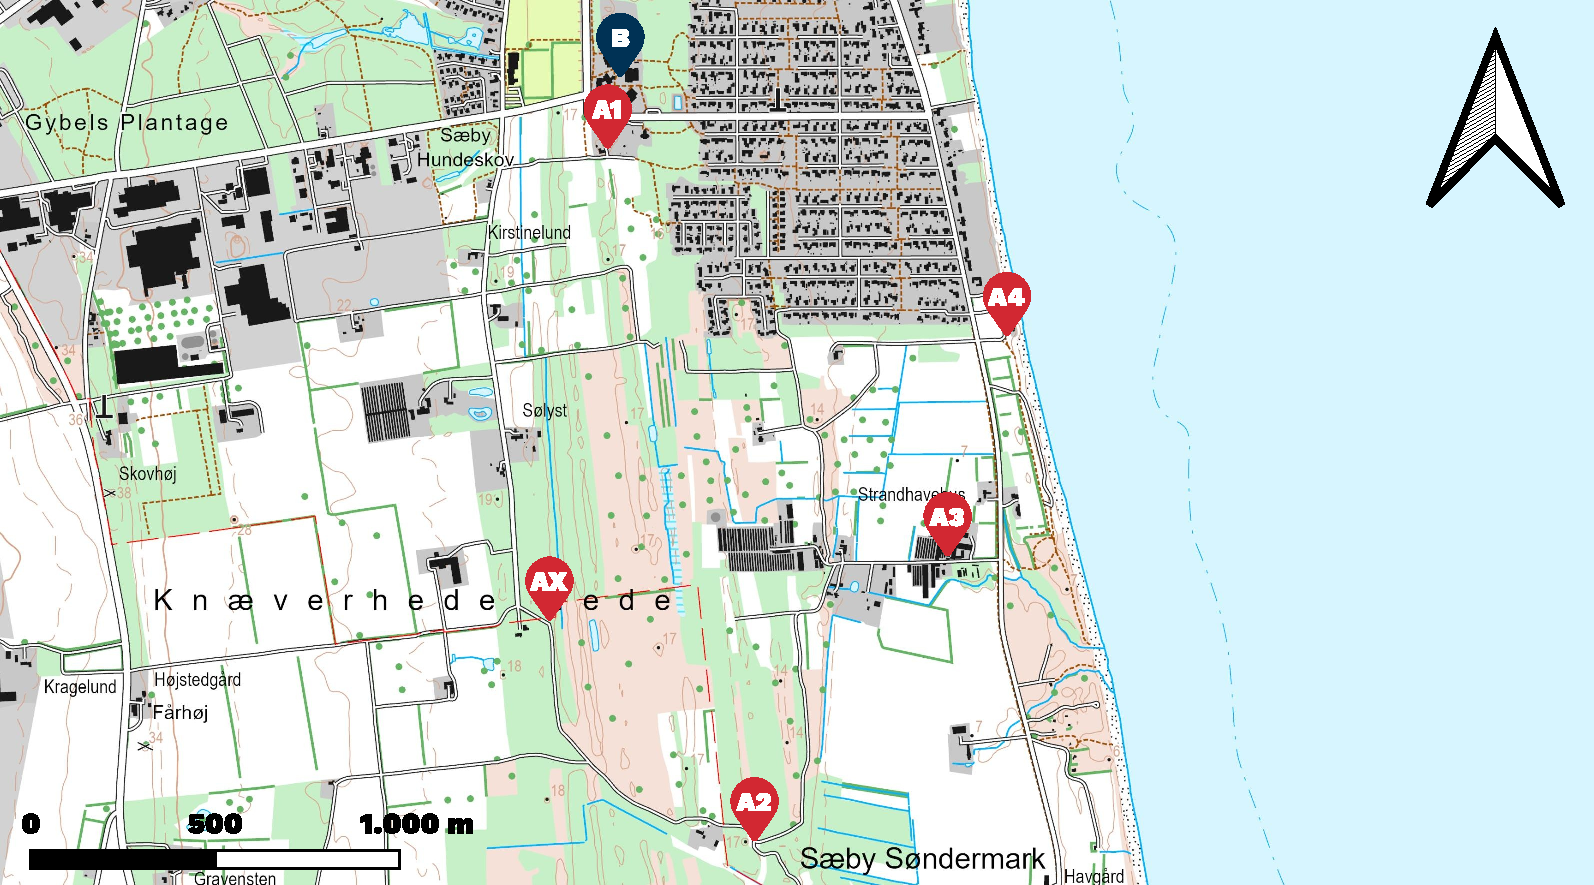
\includegraphics{Kort/RuteA.pdf}
\end{figure}

\newpage
\title{\textcolor{søblå}{Rute B}}
\vspace{0.8cm}
\begin{figure}[H]
    \centering
    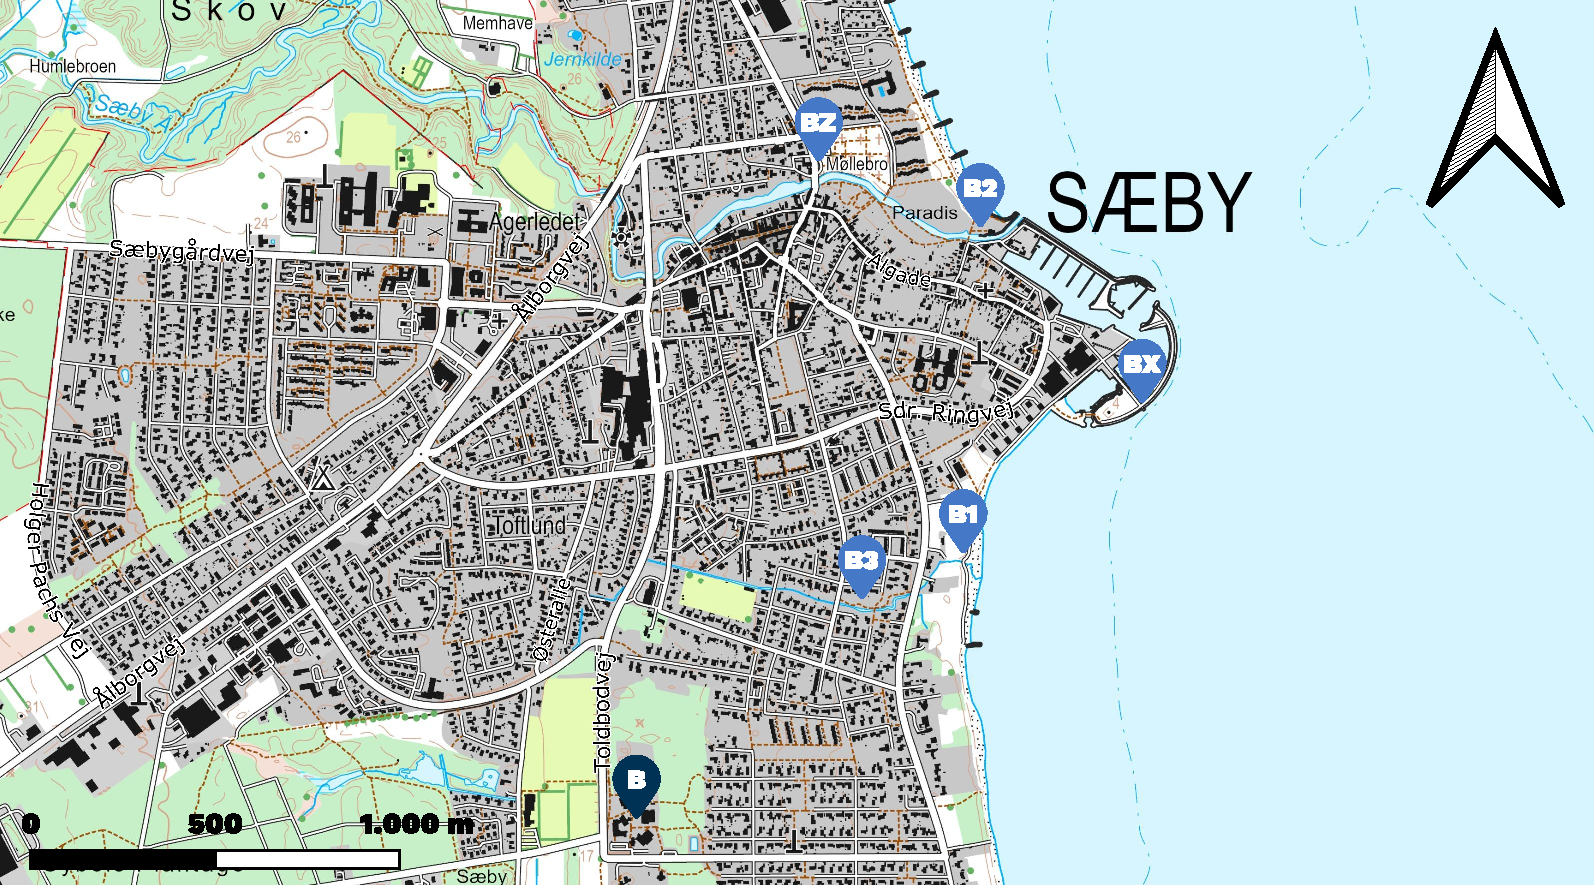
\includegraphics{Kort/RuteB.pdf}
\end{figure}

\newpage
\title{\textcolor{korngul}{Rute C}}
\vspace{0.8cm}
\begin{figure}[H]
    \centering
    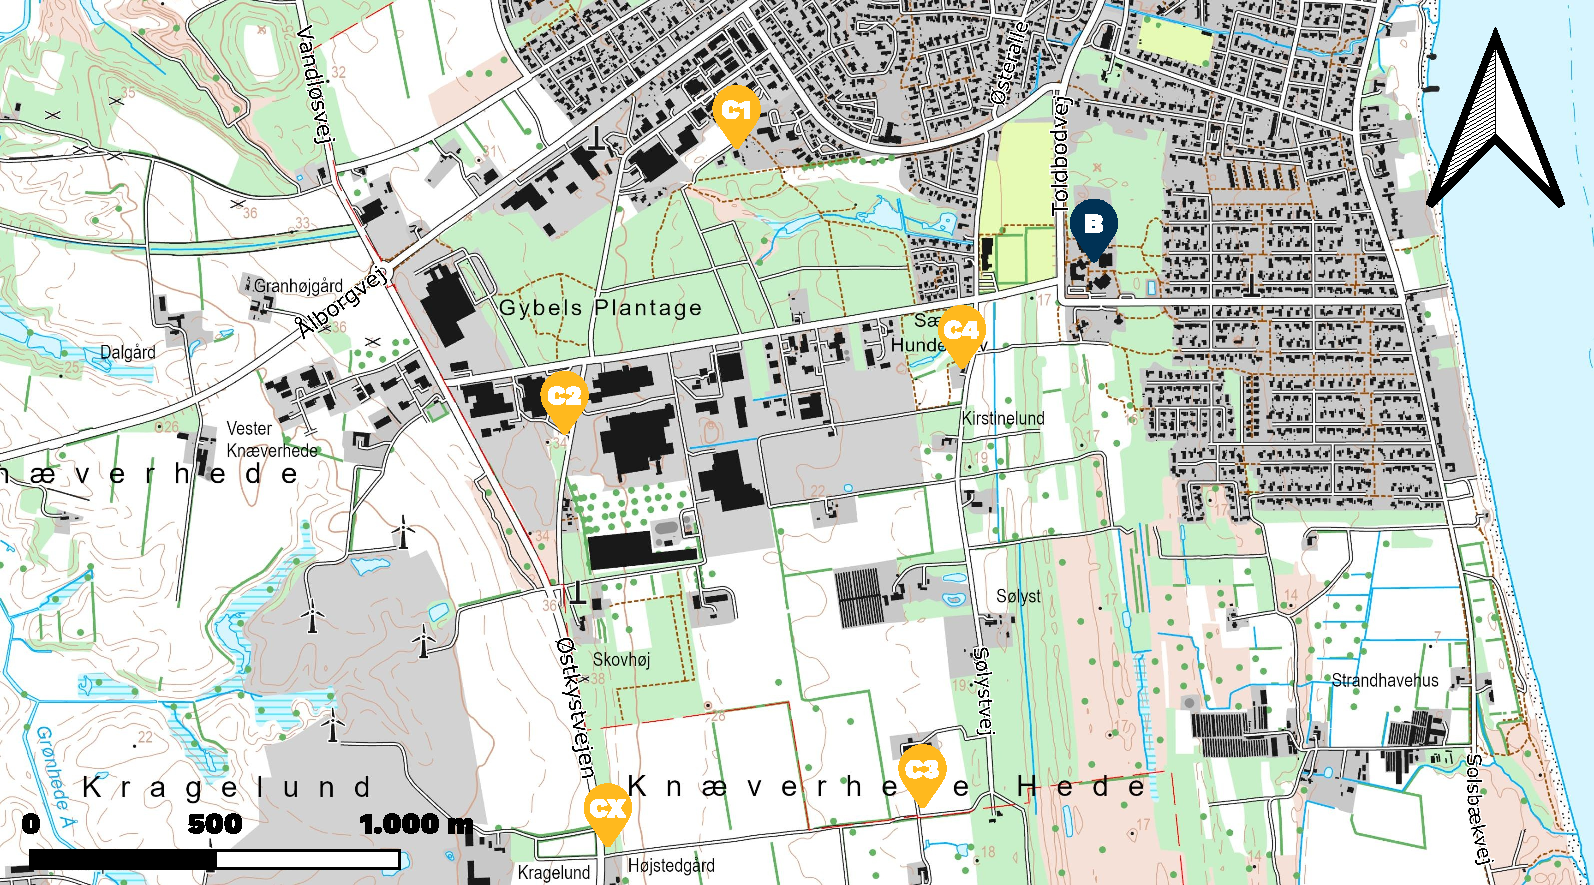
\includegraphics{Kort/RuteC.pdf}
\end{figure}

\newpage
\title{\textcolor{græsgrøn}{Rute D}}
\vspace{0.8cm}
\begin{figure}[H]
    \centering
    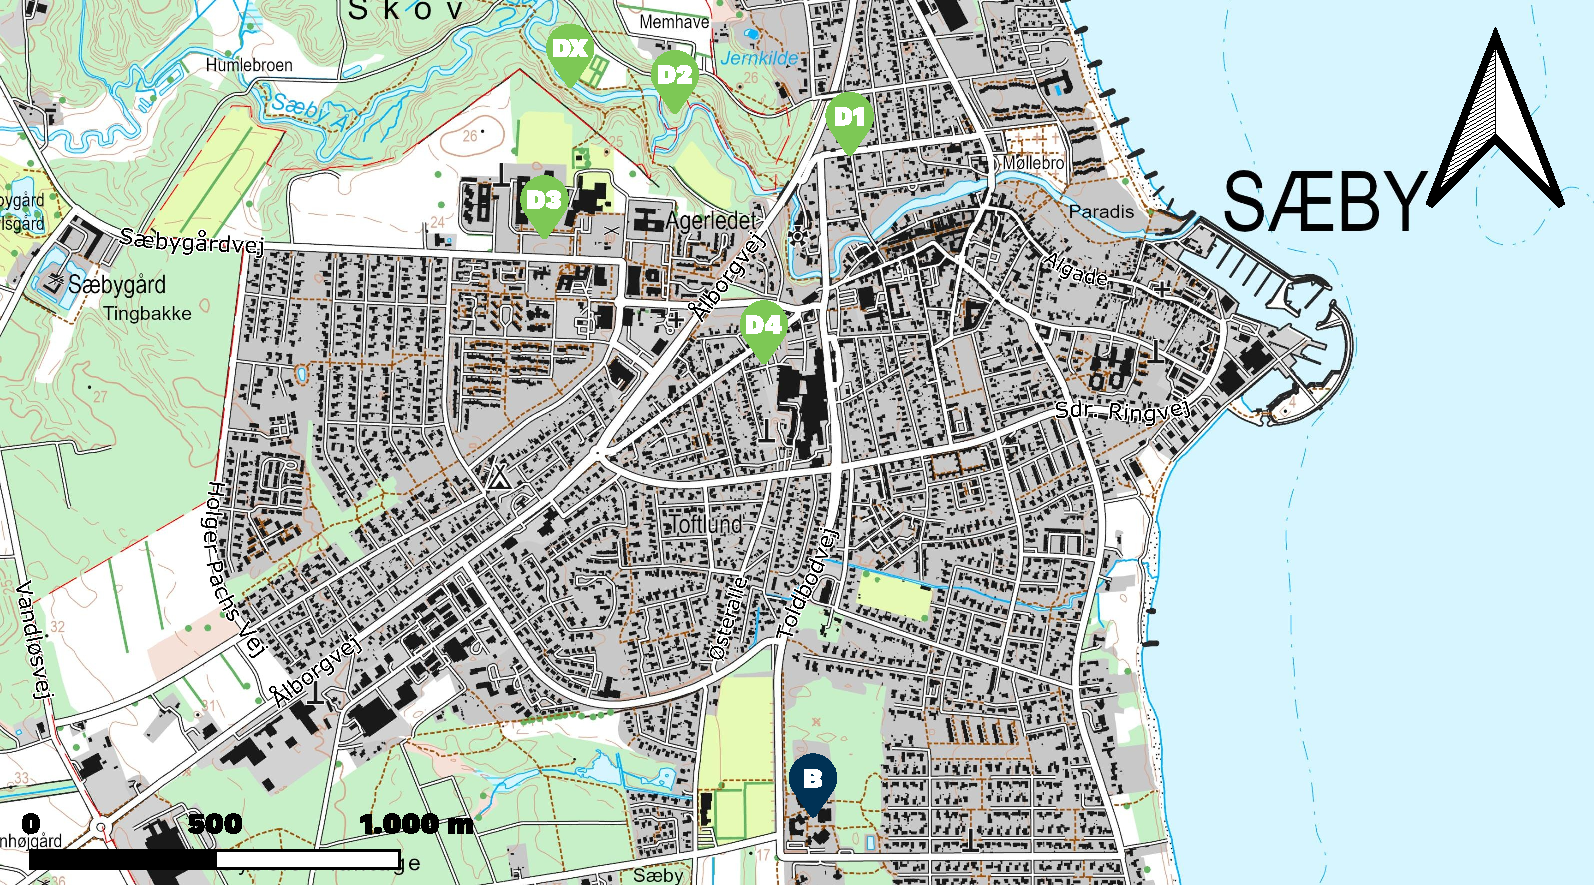
\includegraphics{Kort/RuteD.pdf}
\end{figure}

\end{document}